\section{Design}
\label{design}

The objective of this project is to automatically generate a method-call sequence for a given desired object state. Figure~\ref{fig:mut} shows a method under test of the class \CodeIn{UndirectedDepthFirstSearchAlgorithm} of the QuickGraph library. To cover Statement 9 in the method under test, the field \CodeIn{VisitedGraph} should include edges. Currently, without any assistance Pex cannot cover Statement 9 as it is non-trivial to generate a graph instance with vertices and edges.

\begin{figure}[t]
\begin{CodeOut}
\begin{alltt}
00:public void Compute(IVertex s) \{
01:\hspace*{0.2in}// init vertices
02:\hspace*{0.2in}foreach(IVertex u in VisitedGraph.Vertices) \{
03:\hspace*{0.3in}Colors[u]=GraphColor.White;
04:\hspace*{0.3in}if (InitializeVertex != null)
05:\hspace*{0.4in}InitializeVertex(this, new VertexEventArgs(u));
06:\hspace*{0.2in}\}
07:\hspace*{0.2in}//init edges
08:\hspace*{0.2in}foreach(IEdge e in VisitedGraph.Edges) \{
09:\hspace*{0.3in}EdgeColors[e]=GraphColor.White;
10:\hspace*{0.2in}\}
11:\hspace*{0.2in}// use start vertex
12:\hspace*{0.2in}if (s != null) \{
13:\hspace*{0.3in}if (StartVertex != null)
14:\hspace*{0.4in}StartVertex(this,new VertexEventArgs(s));
15:\hspace*{0.3in}Visit(s);
16:\hspace*{0.2in}\}
17:\hspace*{0.2in}// visit vertices
18:\hspace*{0.2in}foreach(IVertex v in VisitedGraph.Vertices) \{
19:\hspace*{0.3in}if (Colors[v] == GraphColor.White) \{
20:\hspace*{0.4in}if (StartVertex != null)
21:\hspace*{0.5in}StartVertex(this,new VertexEventArgs(v));
22:\hspace*{0.3in}Visit(v);
23:\hspace*{0.2in}\}
24:\hspace*{0.2in}\}
25:\}
\end{alltt}
\end{CodeOut}
\Caption{\label{fig:mut} A method under test from the QuickGraph library.}
\end{figure}

\subsection{Capture the desired object state}

The first step of our approach is to capture the desired object state (with respect to fields in object types) from the branch that is not covered in the method under test. Figure~\ref{fig:condition} shows the object state captured by the current SeqEx approach. The field that is actually responsible for not able to cover the branch is \CodeIn{ArrayList.\_size}. First, it has to be identified that the uncovered branch (Statement 9) in the method under test is due to the desired condition shown in Figure~\ref{fig:condition}. We can use the approach Covana (developed by Xusheng) to address this issue. We next explain how to generate a method-call sequence for achieving the desired object state.

\begin{figure*}[t]
\begin{CodeOut}
\begin{alltt}
Code location: System.Collections.ArrayList+ArrayListEnumeratorSimple.MoveNext at 0x003e
field: System.Collections.ArrayList._size
field: System.Collections.CollectionBase.list
field: QuickGraph.Representations.AdjacencyGraph.m_Edges
field: QuickGraph.Algorithms.Search.UndirectedDepthFirstSearchAlgorithm.m_VisitedGraph
path condition term: 
UndirectedDepthFirstSearchAlgorithm s7 = new;
AdjacencyGraph s6
   = target == s7 ? g_iVertexAndEdgeListGraph : (AdjacencyGraph)(target.m_VisitedGraph);
AdjacencyGraph s5 = s6;
EdgeCollection s8 = new;
EdgeCollection s4 = s5 == (AdjacencyGraph)s7 ? s8 : s5.m_Edges;
EdgeCollection s3 = s4;
EdgeCollection s2 = s3 == s8 ? s8 : (EdgeCollection)(((CollectionBase)s3).list);
EdgeCollection s1 = s2;
int s0 = s1 == s8 ? 0 : ((ArrayList)s1).\_size;
return -1 < -1 + s0;
\end{alltt}
\end{CodeOut}
\Caption{\label{fig:condition} Desired object state captured by the current SeqEx approach.}
\end{figure*}

\subsection{Identifying methods of interest}

Our approach will next identify the methods that modify the fields captured in the desired object state. To address this issue, we need several types of information, which can be gathered either dynamically or statically. In our approach, We plan to use a combination of dynamic and static analyses for achieving this purpose. The advantage of using dynamic analysis is that captured information is precise. However, only a limited information can be captured as dynamic analysis requires the relevant portions of the code to be executed. On the other hand, the information captured using static analysis is imprecise due to its conservative nature.

In our approach, we need to capture the following types of information:

\begin{itemize}
\item Modified Fields: Includes information of which fields are modified by different methods of classes in the application under analysis. Useful for detecting the methods of interest.
\item Read Fields: Includes information of which fields are read by different methods. This is useful to detect dependencies among methods.
\item Caller/Callee Methods: Includes information of methods called by different methods.
\end{itemize}

Using \emph{Modified Fields}, it is possible to identify the methods that affect the \CodeIn{\_size} field as \CodeIn{Add} and \CodeIn{Remove} methods of the \CodeIn{ArrayList} class. In total, there are $0$ methods that modify the \CodeIn{\_size} field. It is required to identify which method to choose for achieving desired object state. We plan to use two techniques to precisely choose the method to achieve desired object state.

The first technique is to prune out the methods of the \CodeIn{ArrayList} class that are not invoked by its callers in the application under analysis. 
However, these methods cannot be directly invoked as the instance of the \CodeIn{ArrayList} class is not visible outside. Therefore, it is required to identify the object (which is visible) and also the method of the instance, which can be invoked. We plan to use the \emph{Called/Callee Methods} information to address this issue. More specifically, we construct a directed graph as shown in Figure~\ref{}. The objective of our algorithm is to identify an object whose level is as minimum as possible and an associated method of the object that 

%%%%%%%%%%%%%%%%%%%%%%%%%%%%%%%%%%%%%%%%%%%%%%%%%%%%%%%%%%%%%%%%%%%%%%%%%%%%%%%%%%%%%%%%%%%%%%%%%%%%%%%%%%%%%%%%
% PREVIOUS DESIGN BASED ON CONSTRAINT SOLVING

%The objective of this project is to automatically generate a method-call sequence for a given desired object state. Figure~\ref{fig:simplestack} shows a simple stack implementation. Figure~\ref{fig:mut} shows a method under test using the \CodeIn{SimpleStack}. To cover the \CodeIn{true} branch of the \CodeIn{if} method, the desired object state is to have more than five elements in the stack. The desired method-call sequence for achieving this desired object state is to create an instance of \CodeIn{SimpleStack} and invoke the \CodeIn{Push} method for six or more times. We next explain our proposed approach in detail.
%
%\begin{figure}[t]
%\begin{CodeOut}
%\begin{alltt}
%public class SimpleStack \{
%\hspace*{0.2in}int count;
%\hspace*{0.2in}int[] elements;
%\hspace*{0.2in}int currentPosition;
%\hspace*{0.2in}public SimpleStack() \{
%\hspace*{0.3in}elements = new int[20];
%\hspace*{0.3in}currentPosition = 0;
%\hspace*{0.3in}count = 0;
%\hspace*{0.2in}\}
%
%\hspace*{0.2in}public void Push(int i) \{
%\hspace*{0.3in}if (currentPosition >= 20)
%\hspace*{0.4in}throw new Exception("Stack full");
%\hspace*{0.3in}elements[currentPosition++] = i;
%\hspace*{0.3in}count++;
%\hspace*{0.2in}\}
%
%\hspace*{0.2in}public int Pop() \{
%\hspace*{0.3in}if (currentPosition == 0)
%\hspace*{0.4in}throw new Exception("Stack empty");
%\hspace*{0.3in}count--;
%\hspace*{0.3in}return elements[--currentPosition];
%\hspace*{0.2in}\}
%
%\hspace*{0.2in}public int Size() \{
%\hspace*{0.3in}return count;
%\hspace*{0.2in}\}
%\}
%\end{alltt}
%\end{CodeOut}
%\Caption{\label{fig:simplestack} Simple Stack Implementation.}
%\end{figure}
%
%\begin{figure}[t]
%\begin{CodeOut}
%\begin{alltt}
%\hspace*{0.2in}public void MUT(SimpleStack st) \{
%\hspace*{0.3in}if (st.Size() > 5) \{
%\hspace*{0.4in}...
%\hspace*{0.2in}\}
%\}
%\end{alltt}
%\end{CodeOut}\vspace*{-3ex}
%\Caption{\label{fig:mut} Method under test.}\vspace*{-3ex}
%\end{figure}
%
%\subsection{Capture desired object state}
%
%When a particular branch in the code under test is not covered, our approach will precisely capture the desired object state (with respect to fields in object types) from the branch that is not covered in the code under test. For example, in our method under test, the desired object state should be the field \CodeIn{count} of \CodeIn{SimpleStack} should be greater than five. 
%
%The desired object state can be more complex and often lead to another desired object state. For example, consider another class under test \CodeIn{InternalFields} (Figure~\ref{fig:iftest}) and MUT (Figure~\ref{fig:iftest}). In this scenario, the desired state is the field \CodeIn{localState} should be \CodeIn{true}. However, the local state is set to \CodeIn{true} in the method \CodeIn{SetLocalState} (a \CodeIn{private} method) when other fields are in certain desired object state such as \CodeIn{member1 == 5}, \CodeIn{member2 == 3}, and \CodeIn{member3 $>$ 2}. This example illustrates a chaining scenario while capturing the desired object state. In particular, addressing one desired object state can lead to multiple desired states that need to be further addressed.
%
%\begin{figure}[t]
%\begin{CodeOut}
%\begin{alltt}
%\emph{InternalFields CUT}
%public class InternalFields \{
%\hspace*{0.2in}private int member1, member2, member3;
%\hspace*{0.2in}private bool localState;
%\hspace*{0.2in}public bool InternalState \{
%\hspace*{0.3in}get \{
%\hspace*{0.4in}return localState;
%\hspace*{0.3in}\}
%\hspace*{0.2in}\}
%\hspace*{0.2in}private void SetLocalState() \{
%\hspace*{0.3in}if (member1 == 5 && member2 == 3 && member3 > 2)
%\hspace*{0.4in}localState = true;
%\hspace*{0.2in}\}
%\hspace*{0.2in}public void IncrM1() \{
%\hspace*{0.3in}member1++;
%\hspace*{0.3in}SetLocalState();
%\hspace*{0.2in}\}
%\hspace*{0.2in}public void IncrM2AndDecrM1() \{
%\hspace*{0.3in}member2++;
%\hspace*{0.3in}member1--;
%\hspace*{0.3in}SetLocalState();
%\hspace*{0.2in}\}
%\hspace*{0.2in}public void IncrM3AndDecrM1() \{
%\hspace*{0.3in}member3++;
%\hspace*{0.3in}member1--;
%\hspace*{0.3in}SetLocalState();
%\hspace*{0.2in}\}   
%\}
%\emph{Method Under Test}
%public void FieldCheck(InternalFields ifd) \{
%\hspace*{0.2in}if (ifd.InternalState) \{
%\hspace*{0.3in}...
%\hspace*{0.2in}\}
%\}
%\end{alltt}
%\end{CodeOut}
%\Caption{\label{fig:iftest} InternalFields Class and a method under test based on this class.}
%\end{figure}
%
%\subsection{Identifying methods of interest}
%
%Our approach will next identify the methods of the class under test that modify the fields captured in the desired object state. For example, in the case of \CodeIn{SimpleStack}, our approach will identify that the \CodeIn{count} field is modified by the methods \CodeIn{Push} and \CodeIn{Pop}. Similarly, in the case of \CodeIn{InternalFields}, our approach will identify that \CodeIn{member1} is modified by \CodeIn{IncrM1}, \CodeIn{IncrM2AndDecrM1}, and \CodeIn{IncrM3AndDecrM1}. Our approach will next identify how many times each method has to be invoked. 
%
%To address this issue, our approach will first generate conditional terms (suitable for solving via a constraint solver) that represent the desired object state in terms of method calls. For example, the field \CodeIn{count} is increased by the \CodeIn{Push} method and is decreased by the \CodeIn{Pop} method. Lets consider that ``X'' represents the number of times the \CodeIn{Push} method has to be called and ``Y'' represents the number of times the \CodeIn{Pop} method has to be called. The equation for the \CodeIn{count} field to achieve desired object state is ``X - Y $>$ 5''. There can be multiple equations based on the desired object state.
%
%For the \CodeIn{InternalFields} class, to achieve the desirable object, the method \CodeIn{SetLocalState} has to be invoked once. Therefore, the terms for achieving this state are ``S == 1'', where S represents the number of times the method \CodeIn{SetLocalState} has to be invoked. However, invoking this method simply does not achieve the desired object state as it requires another state to be achieved for covering the \CodeIn{true} branch of the \CodeIn{SetLocalState} method. This chaining of desired states  can be identified by executing the current sequence and by discovering new branches that are not covered. Our approach will next construct more terms that represent the new state to be achieved. Consider that ``X'' represents the number of times \CodeIn{IncrM1} has to be invoked, ``Y'' represents the number of times \CodeIn{IncrM2AndDecrM1} has to be invoked, and ``Z'' represents the number of times \CodeIn{IncrM3AndDecrM1} has to be invoked. The terms for achieving desired object state are as follows:
%
%\begin{center}
%\begin{CodeOut}
%\begin{alltt}
%S == 1
%X - Y - Z == 5
%Y == 3
%Z > 2
%\end{alltt}
%\end{CodeOut}
%\end{center}
%
%Using constraint solver, these terms can be solved to get concrete values for fields S, X, Y, and Z. These concrete values represent the number of times the associated method calls has to be invoked to achieve desired object states. In our current example, a constraint solver can return values for S, X, Y, and Z as 1, 11, 3, and 3, respectively. Based on this information, it can be inferred that an example desired method-call sequence can be as follows:
%
%\begin{CodeOut}
%\begin{alltt}
%InternalFields internalFields = new InternalFields();
%for(int c1 = 0; c1 < 11; c1++)
%\hspace*{0.3in}internalFields.IncrM1();
%for (int c2 = 0; c2 < 3; c2++)
%\hspace*{0.3in}internalFields.IncrM2AndDecrM1();
%for (int c3 = 0; c3 < 3; c3++)
%\hspace*{0.3in}internalFields.IncrM3AndDecrM1();            
%return internalFields;
%\end{alltt}
%\end{CodeOut}
%
%\subsection{Getting an instance of class under test}
%
%Existing approaches such as Prospector~\cite{prospector:jungloid} or JCrasher~\cite{csallner:jcrasher} can be used to identify how to get an instance of the desired class under test. These approaches constructs a graph, referred to as signature graph, from the signatures of APIs. This signature graph helps to get an instance of the target class under test. Although these approaches help in getting target class under test, these approaches do not help in generating desired object state for the class under test. More specifically, their signature graphs often do not include the state-modifying methods of the class under test.
%
%\subsection{Inferring specification of class under test}
%
%It is often not sufficient to identify what are the methods of interest, since there can be several dependencies among methods. Due to those dependencies, it is often possible that the generated method-call sequences are not valid (i.e., they may result in compilation errors or throw run-time exceptions). For example, we also need information on the sequence of how to invoke the identified methods under test. Furthermore, it is required to capture any additional methods that have to be invoked before invoking the identified methods under test. For example, consider a variant of the class \CodeIn{InternalFields} shown in Figure~\ref{fig:iftest1}, which is more simpler than the original class. It is easy to identify that the desired object state can be achieved by invoking the method \CodeIn{IncrM1} five times. However, the method \CodeIn{IncrM2} should also be called five times along with the method \CodeIn{IncrM1}. Inferring specifications for the class under test can help address these issues. For example, a simple specification in terms of the finite automaton for the \CodeIn{MultiMethodsInLoop} is shown in Figure~\ref{fig:loopfsa}. The specification describes several aspects such as \CodeIn{IncrM2} should be called before \CodeIn{IncrM1}. The specification also shows that \CodeIn{IncrM2} should be called after \CodeIn{IncrM1} before invoking \CodeIn{IncrM1} again.
%
%\begin{figure}[t]
%\begin{CodeOut}
%\begin{alltt}
%public class MultiMethodsInLoop \{
%\hspace*{0.2in}private int member1, member2, member3;
%\hspace*{0.2in}private bool localState;
%\hspace*{0.2in}bool m1set = true, m2set = false;
%        
%\hspace*{0.2in}public bool InternalState \{
%\hspace*{0.3in}get \{
%\hspace*{0.4in}return localState;
%\hspace*{0.3in}\}
%\hspace*{0.2in}\}
%
%\hspace*{0.2in}private void SetLocalState() \{
%\hspace*{0.3in}if (member1 == 5)
%\hspace*{0.4in}localState = true;
%\hspace*{0.2in}\}
%
%\hspace*{0.2in}public void IncrM1() \{
%\hspace*{0.3in}if (!m2set)
%\hspace*{0.4in}throw new Exception("Member2 is not set properly");
%\hspace*{0.3in}member1++;
%\hspace*{0.3in}SetLocalState();
%\hspace*{0.3in}m1set = true;
%\hspace*{0.3in}m2set = false;
%\hspace*{0.2in}\}
%
%\hspace*{0.2in}public void IncrM2() \{
%\hspace*{0.3in}if (!m1set)
%\hspace*{0.4in}throw new Exception("Member1 is not set properly");
%\hspace*{0.3in}m2set = true;
%\hspace*{0.3in}m1set = false;
%\hspace*{0.2in}\}
%\}
%\end{alltt}
%\end{CodeOut}
%\Caption{\label{fig:iftest1} \CodeIn{MultiMethodsInLoop} Class, which is a variant of \CodeIn{InternalFields}.}
%\end{figure}
%
%\begin{figure}[t]
%\centering
%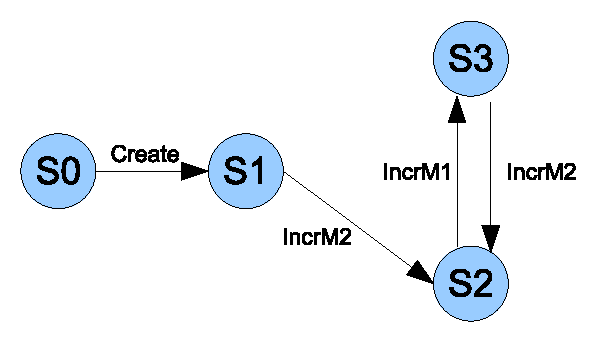
\includegraphics[scale=0.60,clip]{figs/MultiMethodsLoopFsa1.eps}
%\caption{\label{fig:loopfsa}Finite automaton for MultiMethodsLoop class.}
%\end{figure}
%
%These specifications can be inferred either by applying mining approaches on existing code bases~\cite{thummalapenta09:mseqgen} or from the implementation of the class under test~\cite{whaley02:interface}. Inferring complete specifications for all methods of the class under test can itself be a challenging problem that need to be addressed. For example, the approaches that infer specifications from the implementation are not scalable in practice. On the other hand, the approaches that infer specifications using mining approaches may not be able to infer specification for a method if that method is not used by any existing code bases. Therefore, a synergy of these two approaches can help effectively infer specifications.
%
%\subsection{Using specification for sequence generation}
%
%Our approach will next generate sequences that achieve desirable object states based on the inferred specification and the methods of interest. As we already know the methods of interest, the automaton representing can be pruned by not covering those paths that do not include our methods of interest. Next, our approach will explore this automaton to achieve the desired object state by visiting each method as desired number of times.
%
%\subsection{Open Problems}
%
%The current design is based on an assumption that it is possible to infer method summaries, which describe how methods of a class under test are modifying its fields. However, in case of classes from external libraries, it may not be possible to infer method summaries. 